\documentclass[12pt,a4paper]{article}
\usepackage[utf8]{inputenc}
\usepackage[T1]{fontenc}
\usepackage{geometry}
\usepackage{titlesec}
\usepackage{hyperref}
\usepackage{graphicx}
\usepackage{fancyhdr}
\usepackage{enumitem}
\usepackage{tabularx}
\usepackage{longtable}
\usepackage{float}
\usepackage{pdflscape}
\geometry{left=2.5cm,right=2.5cm,top=2.5cm,bottom=2.5cm}
\setlength{\headheight}{15pt}

\pagestyle{fancy}
\fancyhf{}
\fancyhead[L]{S-007: Renewal \& Upsell Advisor}
\fancyhead[R]{Comprehensive SRS}
\fancyfoot[C]{\thepage}

\title{\textbf{Software Requirements Specification}\\ \vspace{1cm} \Large Renewal \& Upsell Advisor\\ \vspace{0.5cm} \large Consolidated Documentation}
\author{}
\date{Version: 2.0\\ \today}

\begin{document}

\maketitle
\thispagestyle{empty}
\begin{center}
    \textbf{Confidential}
\end{center}

\newpage

\tableofcontents

\newpage

\section{Scope}

\subsection{In-Scope}
\begin{itemize}
    \item \textbf{Renewal Risk Management:}
    \begin{itemize}
        \item Contract expiration tracking and automated alerts
        \item Multi-factor churn prediction using ML models
        \item Customer health scoring based on usage, engagement, and sentiment
        \item Risk segmentation (High, Medium, Low) with confidence scores
    \end{itemize}
    \item \textbf{Upsell \& Cross-sell Intelligence:}
    \begin{itemize}
        \item Product adoption and feature usage analysis
        \item Revenue expansion opportunity identification
        \item Cross-sell recommendations based on customer profile and behavior
        \item Whitespace analysis for untapped product offerings
    \end{itemize}
    \item \textbf{Automated Playbook Recommendations:}
    \begin{itemize}
        \item Personalized renewal and expansion plays
        \item Multi-channel outreach cadence suggestions (Email, Phone, Meeting)
        \item Value messaging templates tailored to customer pain points and outcomes
        \item Best-action recommendations with success probability scores
    \end{itemize}
    \item \textbf{Integration Capabilities:}
    \begin{itemize}
        \item Primary: Salesforce CRM, Stripe/Chargebee billing platforms, Google Analytics/Mixpanel
        \item Secondary: Customer Success platforms (Gainsight, ChurnZero), Email (Gmail, Outlook), Product analytics tools
        \item Webhook-based real-time data synchronization
    \end{itemize}
    \item \textbf{Analytics \& Reporting:}
    \begin{itemize}
        \item Renewal forecast dashboard with ARR projections
        \item Pipeline health metrics and trend analysis
        \item Agent performance tracking and recommendation outcomes
        \item Executive summary reports with KPI visualization
    \end{itemize}
\end{itemize}

\subsection{Out-of-Scope}
\begin{itemize}
    \item Contract negotiation and legal document generation
    \item Direct payment processing and transaction handling
    \item Customer onboarding and implementation workflows
    \item Product roadmap planning and feature prioritization
    \item Marketing campaign creation and execution
    \item Technical support ticket management
    \item Full financial accounting and revenue recognition
    \item Integration with non-B2B SaaS business models (e.g., e-commerce, retail)
    \item Manual override of contract terms or pricing
    \item Real-time voice call monitoring and transcription
\end{itemize}

\section{Functional Requirements}

\subsection{FR-1: Contract \& Renewal Tracking}
\subsubsection{FR-1.1: Contract Data Ingestion}
\begin{itemize}
    \item System SHALL ingest contract data from Salesforce including: contract ID, account name, ARR/MRR, start date, end date, renewal date, contract terms
    \item System SHALL automatically sync contract updates within 5 minutes of changes in source system
    \item System SHALL support bulk import of historical contract data (minimum 5 years)
\end{itemize}
\subsubsection{FR-1.2: Renewal Timeline Monitoring}
\begin{itemize}
    \item System SHALL track all contracts with renewal dates within 90-day window
    \item System SHALL automatically create renewal opportunity records in Salesforce 90 days before expiration
    \item System SHALL categorize renewals by time horizon: Immediate (0-30 days), Near-term (31-60 days), Future (61-90 days)
\end{itemize}

\subsection{FR-2: Churn Risk Prediction}
\subsubsection{FR-2.1: Risk Scoring Model}
\begin{itemize}
    \item System SHALL calculate renewal risk score (0-100) for each account using ML model
    \item Risk score SHALL incorporate features: product usage (login frequency, feature adoption), support metrics (ticket volume, resolution time), payment history (late payments, failed charges), engagement (email opens, meeting attendance), sentiment (NPS, survey responses)
    \item \textbf{System SHALL update relationship scores and churn predictions on the entire dataset every 24 hours.}
    \item System SHALL provide 85\% prediction accuracy (validated on historical data)
\end{itemize}
\subsubsection{FR-2.2: Risk Segmentation}
\begin{itemize}
    \item System SHALL classify accounts into risk categories:
    \begin{itemize}
        \item High Risk: Score 70-100 (churn probability >50\%)
        \item Medium Risk: Score 40-69 (churn probability 25-50\%)
        \item Low Risk: Score 0-39 (churn probability <25\%)
    \end{itemize}
    \item System SHALL display top 5 risk factors for each account
    \item System SHALL provide confidence intervals for predictions
\end{itemize}
\subsubsection{FR-2.3: Early Warning Alerts}
\begin{itemize}
    \item System SHALL send real-time alerts when account moves to High Risk category
    \item Alerts SHALL include: account name, ARR at risk, risk score, primary risk factors, recommended actions
    \item System SHALL support alert routing rules (assign to CSM, AE, or team lead based on account ownership)
\end{itemize}

\subsection{FR-3: Upsell \& Cross-sell Identification}
\subsubsection{FR-3.1: Expansion Opportunity Detection}
\begin{itemize}
    \item System SHALL identify upsell opportunities based on:
    \begin{itemize}
        \item User license utilization (threshold: >80\% of purchased seats)
        \item Feature usage patterns (high engagement with premium features on basic plan)
        \item API usage limits (approaching rate limits)
        \item Storage consumption (exceeding 75\% of allocated quota)
    \end{itemize}
    \item System SHALL calculate expansion revenue potential for each opportunity
    \item \textbf{Upsell propensity models SHALL be re-evaluated every 24 hours as part of the daily relationship score update.}
    \item System SHALL rank opportunities by expected value and win probability
\end{itemize}
\subsubsection{FR-3.2: Cross-sell Recommendations}
\begin{itemize}
    \item System SHALL recommend complementary products based on:
    \begin{itemize}
        \item Current product usage (collaborative filtering)
        \item Industry segment and company size
        \item Similar customer adoption patterns
    \end{itemize}
    \item System SHALL support whitespace analysis (identify unused products in customer’s plan tier)
\end{itemize}

\subsection{FR-4: Automated Playbook Recommendations}
\subsubsection{FR-4.1: Playbook Library}
\begin{itemize}
    \item System SHALL include minimum 15 pre-built playbooks:
    \begin{itemize}
        \item Renewal Playbooks: High-Risk Intervention, Executive Business Review, Value Realization Workshop, Competitive Displacement Defense
        \item Upsell Playbooks: License Expansion, Feature Upgrade, Multi-Year Commitment, Premium Support Add-on
    \end{itemize}
    \item Each playbook SHALL contain: trigger conditions, outreach cadence (timeline), email/call script templates, success metrics
\end{itemize}

\subsection{FR-5: Outreach Cadence Optimization}
\begin{itemize}
    \item System SHALL recommend outreach sequence across channels: Email, Phone Call, LinkedIn Message, In-Product Notification
    \item System SHALL optimize timing based on: historical engagement patterns, recipient time zone, industry benchmarks
    \item System SHALL support customizable cadence templates (3-touch, 5-touch, 7-touch sequences)
\end{itemize}

\subsection{FR-6: Sentiment \& Engagement Analysis}
\subsubsection{FR-6.1: Sentiment Tracking}
\begin{itemize}
    \item System SHALL analyze sentiment from customer emails using NLP (spaCy, Hugging Face)
    \item System SHALL classify sentiment as Positive, Neutral, Negative with confidence score
    \item \textbf{Sentiment analysis SHALL contribute to the daily (24-hour) relationship score calculation.}
\end{itemize}

\subsection{FR-7: Analytics \& Reporting}
\subsubsection{FR-7.1: Renewal Pipeline Dashboard}
\begin{itemize}
    \item Dashboard SHALL display:
    \begin{itemize}
        \item Total ARR at risk (segmented by risk level)
        \item Renewal rate forecast (current quarter, next quarter)
        \item Top 10 at-risk accounts by ARR
        \item Churn reason analysis (historical)
    \end{itemize}
    \item Dashboard SHALL support filtering by: renewal date range, account segment, assigned CSM/AE
\end{itemize}
\subsubsection{FR-7.2: Relationship Score Visualization}
\begin{itemize}
    \item System SHALL visualize the relationship score and engagement data in a flyout-style dashboard.
    \item The visualization style SHALL follow the design reference shown below:
    
    \begin{figure}[H]
        \centering
        \includegraphics[width=0.9\textwidth]{Engagement-AI-tab-top-half-with-Zendesk-WITH-FLYOUTS-1-1024x562.png}
        \caption{Engagement AI Dashboard Style Reference}
    \end{figure}
\end{itemize}

\section{System Architecture}

\subsection{System Architecture Overview}
The Renewal \& Upsell Advisor follows a microservices architecture. The detailed data flow key components are illustrated below:

\begin{figure}[H]
    \centering
    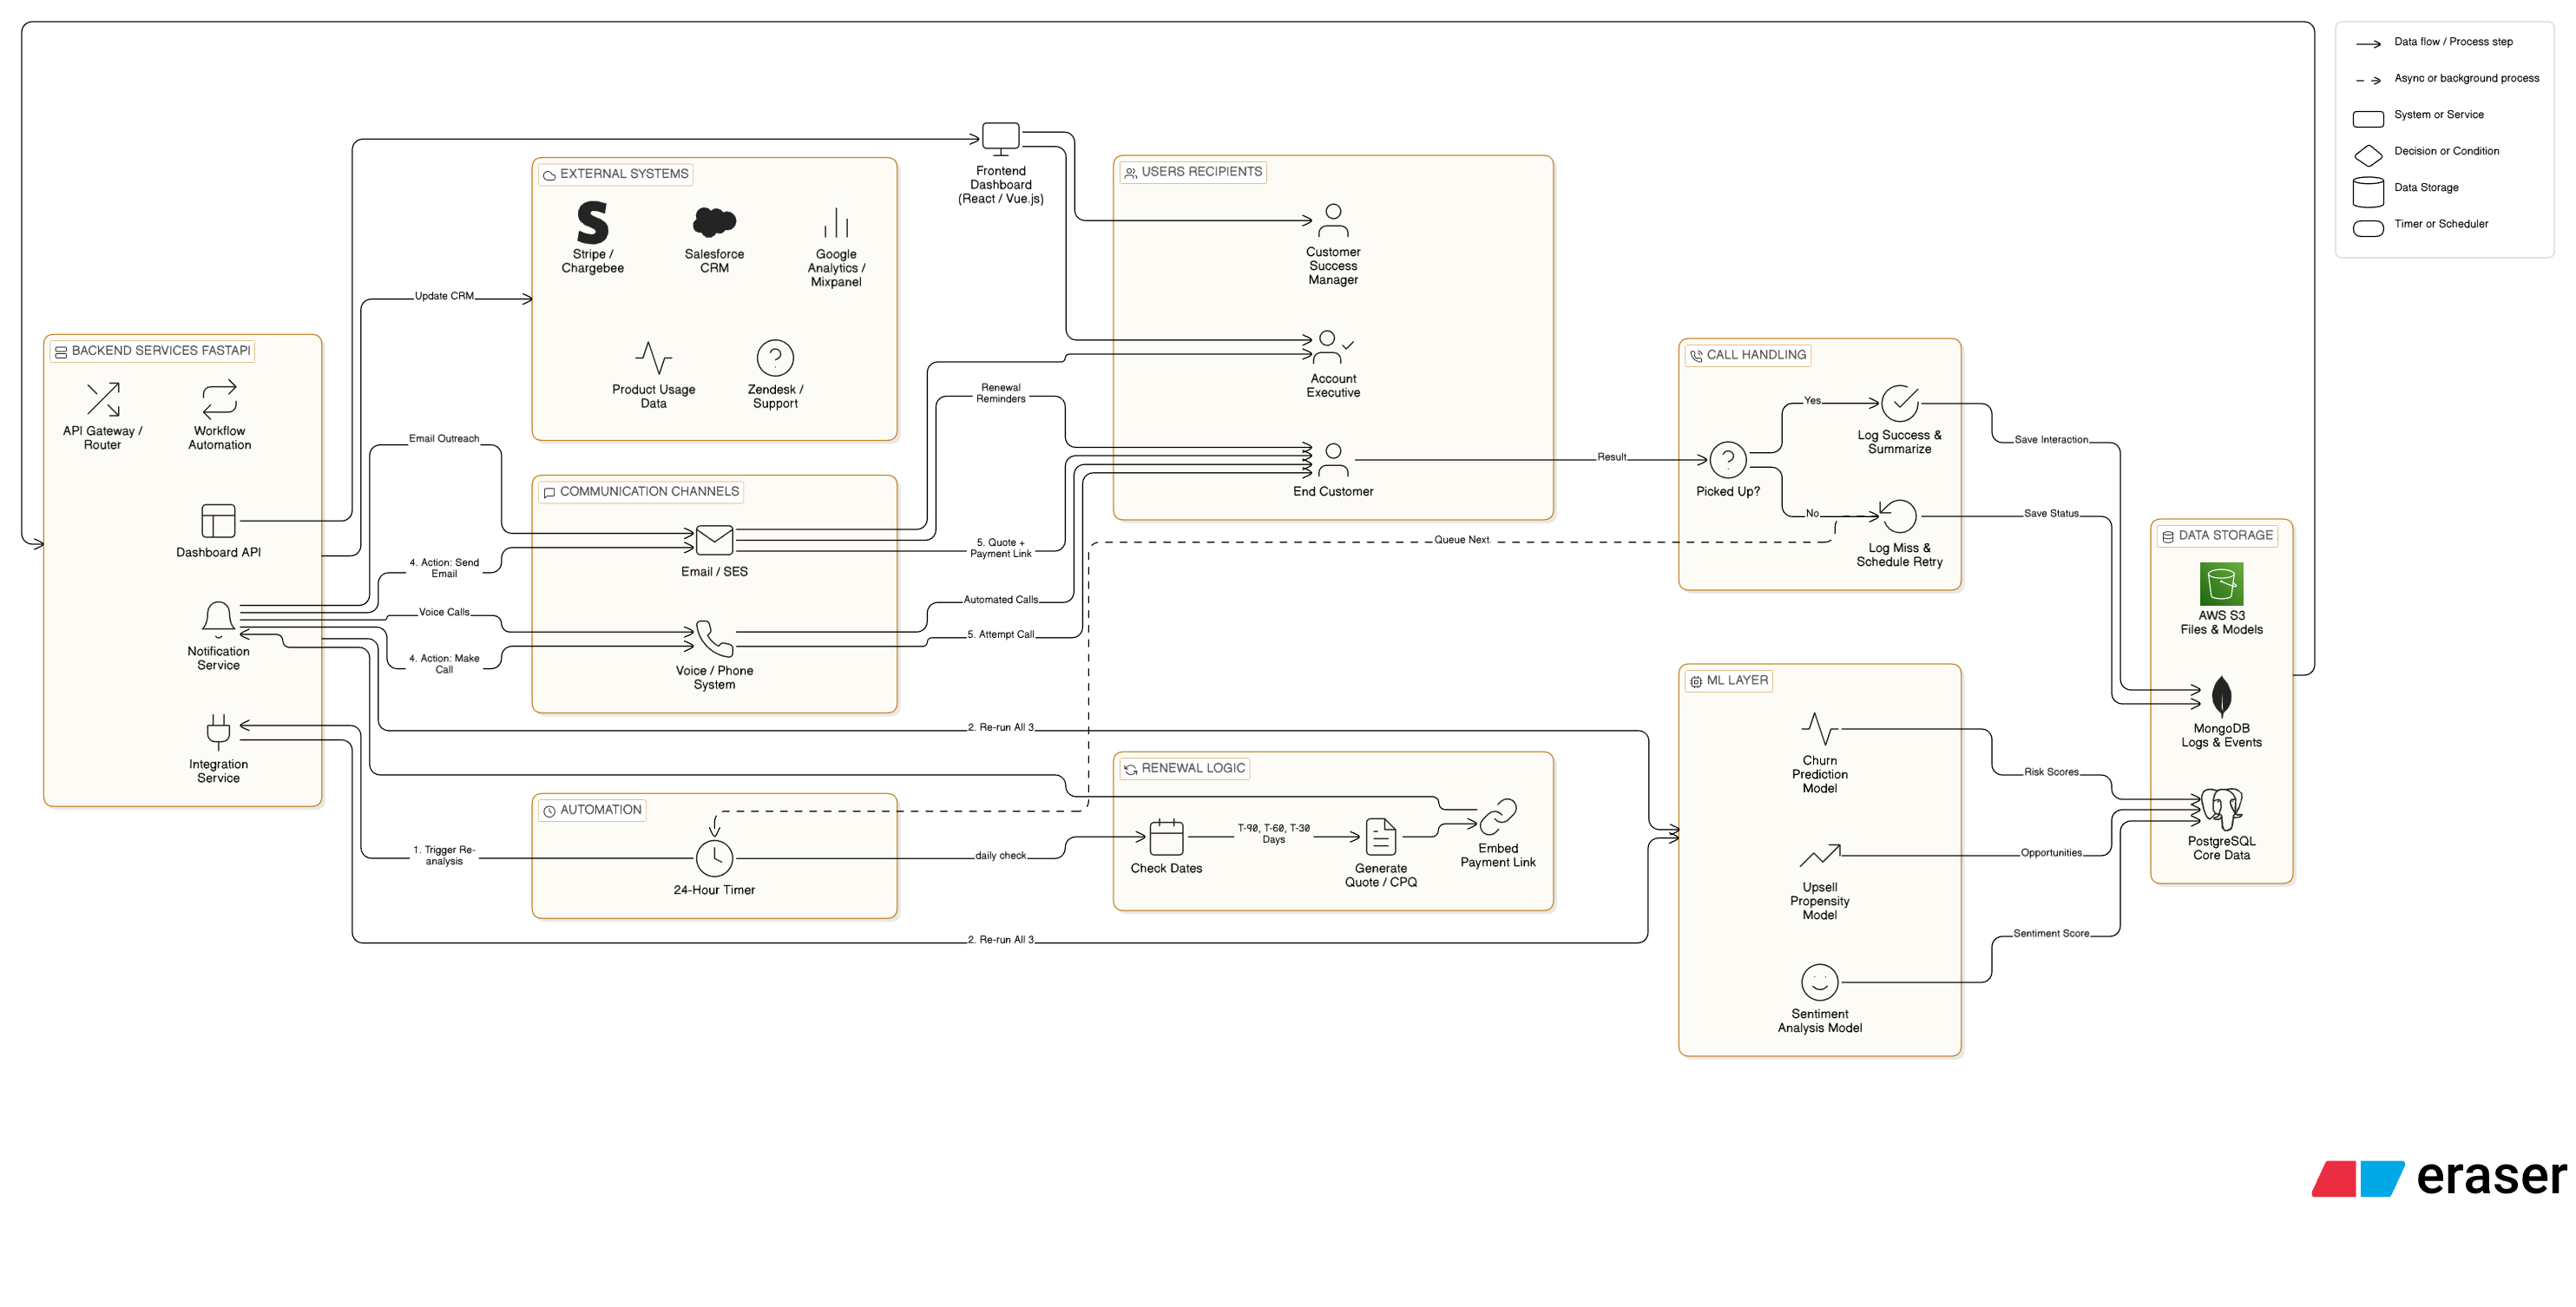
\includegraphics[width=0.9\textwidth]{2.png}
    \caption{System Architecture Diagram - Detailed Data Flow}
\end{figure}

\begin{enumerate}
    \item \textbf{Integration Layer:} Handles bidirectional data synchronization with external systems (Salesforce, Stripe, Analytics platforms)
    \item \textbf{Processing Layer:} Executes data transformation, feature engineering, ML inference, and business logic
    \item \textbf{Presentation Layer:} Provides user interfaces (dashboard) and notification delivery
\end{enumerate}

\subsection{Detailed Autonomous Workflows}

\subsubsection{Workflow 1: The 24-Hour Analysis Loop}
\begin{enumerate}
    \item \textbf{Scheduler Trigger:} A central 24-hour timer triggers the analysis pipeline daily.
    \item \textbf{Re-Analysis:} The system triggers a concurrent re-evaluation of all three primary models for the entire customer base:
    \begin{itemize}
        \item \textbf{Sentiment Analysis:} Re-scans recent emails and support tickets to update the relationship score.
        \item \textbf{Churn Prediction:} Recalculates risk probability based on the latest 24 hours of usage and interaction data.
        \item \textbf{Upsell Propensity:} Re-assesses expansion likelihood based on new feature adoption metrics.
    \end{itemize}
    \item \textbf{Decision Engine:} Updates risk scores and opportunities in the PostgreSQL database.
\end{enumerate}

\subsubsection{Workflow 2: Yagna-Style Renewal Triggers}
\begin{enumerate}
    \item \textbf{Date Verification:} The daily scheduler checks contract expiration dates against specific windows: T-90, T-60, and T-30 days.
    \item \textbf{Automated Action:}
    \begin{itemize}
        \item \textbf{T-90 Days:} Triggers initial "Early Warning" quote generation.
        \item \textbf{T-60 Days:} Regenerates quote with any updated usage metrics.
        \item \textbf{T-30 Days:} Generates "Urgent Renewal" quote.
    \end{itemize}
    \item \textbf{Quote Generation:} The CPQ engine automatically generates a PDF quote and embeds a secure Stripe/Chargebee \textbf{Payment Link} directly into the notification.
    \item \textbf{Delivery:} The quote and payment link are sent to the customer via Email.
\end{enumerate}

\subsubsection{Workflow 3: Closed-Loop Voice Outreach}
\begin{enumerate}
    \item \textbf{Call Attempt:} For high-priority cases, the Voice System initiates an automated call to the customer.
    \item \textbf{Outcome Handling (Decision Node):}
    \begin{itemize}
        \item \textbf{Picked Up:} The AI agent engages in the conversation. The transcript and success status are logged to MongoDB.
        \item \textbf{Missed / No Answer:} The system logs the "Missed" status to MongoDB.
    \end{itemize}
    \item \textbf{Retry Logic:} If the call was missed, the Scheduler automatically queues a \textbf{Retry Attempt} for a later time slot, ensuring no high-value renewal is abandoned after a single failure.
\end{enumerate}

\subsubsection{Workflow 4: Forecast \& Reporting}
\begin{enumerate}
    \item Monthly batch job aggregates all renewals for next quarter
    \item System calculates weighted renewal forecast: (Low Risk ARR $\times$ 95\%) + (Medium Risk $\times$ 75\%) + (High Risk $\times$ 40\%)
    \item Expansion pipeline added to base renewal forecast
    \item Dashboard displays: Total forecasted ARR, Confidence intervals (P10, P50, P90), Risk-adjusted retention rate
    \item Executive report exported to PDF and emailed to VP Sales
\end{enumerate}

\section{Competitive Analysis \& Market Landscape}

\subsection{Market Landscape}
The renewal and upsell intelligence market includes specialized customer success platforms, revenue operations tools, and channel automation platforms. Key competitors include Gainsight, ChurnZero, and Yagna iQ.

\subsection{Competitor Deep Dive: ChurnZero}
\textbf{Product URL:} \url{https://churnzero.com/}

\begin{figure}[H]
    \centering
    \includegraphics[width=0.8\textwidth]{chunrzero1.png}
    \caption{ChurnZero Platform Interface}
    \label{fig:churnzero}
\end{figure}

\subsubsection{Overview}
ChurnZero helps Customer Success teams identify risk and understand relationship health through automated analysis of communications.

\subsubsection{Key Methodologies}
\begin{enumerate}
    \item \textbf{The One-Slide Value Review:} A modern alternative to traditional QBRs.
    \begin{itemize}
        \item \textbf{Expected Value:} Re-anchors conversation on original business goals.
        \item \textbf{Value Delivered:} Focuses on impact (e.g., "Saved 10 hours") rather than activity.
        \item \textbf{Proof of Value:} Data visualizing progress (Baseline $\rightarrow$ Current $\rightarrow$ Target).
        \item \textbf{Next Steps:} Focus on the next 90 days and executive asks.
    \end{itemize}
    \item \textbf{Engagement AI:}
    \begin{itemize}
        \item \textbf{Sentiment Analysis:} Scans emails/surveys to tag interactions as Positive/Neutral/Negative.
        \item \textbf{Topic Tracking:} Identifies themes like "Bugs" or "Pricing" automatically.
        \item \textbf{Relationship Score:} Real-time health signal from communication sentiment.
    \end{itemize}
\end{enumerate}

\subsubsection{CRO Expectations}
\begin{itemize}
    \item CS as a revenue engine responsible for Net Revenue Retention (NRR).
    \item "Objective Health" scores based on actions/adoption rather than subjective feelings.
    \item Tight alignment between Sales promises and CS delivery.
\end{itemize}

\subsection{Competitor Deep Dive: Yagna iQ}
\textbf{Product URL:} \url{https://www.yagnaiq.com/}

\begin{figure}[H]
    \centering
    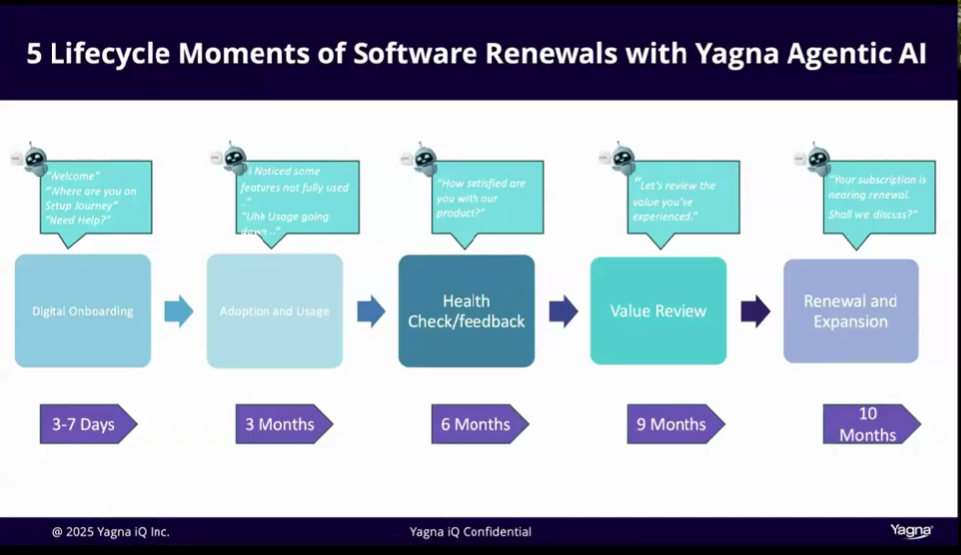
\includegraphics[width=0.8\textwidth]{yagna.png}
    \caption{Yagna iQ Renewal Path Architecture}
    \label{fig:yagna}
\end{figure}

\subsubsection{Platform Overview}
Yagna iQ is a channel ecosystem platform focusing on removing manual processes in distribution channels. It connects Vendors, Distributors, and Resellers.

\subsubsection{Key Modules}
\begin{enumerate}
    \item \textbf{Renewal Cloud (Recurring Revenue Automation):}
    \begin{itemize}
        \item Solves the "1000 Portal Problem" by aggregating multi-vendor data.
        \item \textbf{Zero-Touch Automation:} Proactive renewal quotes sent 90/60/30 days in advance.
        \textbf{ROI:} Claimed to save 125+ hours per 100 contracts and increase on-time renewal rates by 20-25%.
    \end{itemize}
    \item \textbf{XSUS Cloud (Cross-Sell \& Upsell):}
    \begin{itemize}
        \item Uses data mining to identify "Smart Leads" in the install base.
        \item Identifies End-of-Life (EOL) products for tech refresh.
        \item White-space analysis for product attach opportunities.
    \end{itemize}
    \item \textbf{Channel CPQ:}
    \begin{itemize}
        \item Multi-vendor CPQ allowing partners to build complex quotes.
        \item Guided selling and advanced pricing engines.
    \end{itemize}
\end{enumerate}

\subsubsection{Agentic AI Capabilities ("Jana")}
\begin{itemize}
    \item **Natural Language Querying:** "Show me delayed renewals in Asia".
    \item **Automated Quote Editing:** Parses emails to modify and regenerate quotes.
    \item **Voice AI:** Agents that can hold human-like phone conversations for renewals, handling interruptions and distinct accents.
\end{itemize}

\subsection{Competitive Comparison Matrix}
\footnotesize
\setlength{\tabcolsep}{2pt}
\renewcommand{\arraystretch}{1.2}

\begin{longtable}{|p{2.2cm}|p{2.8cm}|p{1.7cm}|p{1.7cm}|p{1.5cm}|p{1.7cm}|p{2.2cm}|}
\hline
\textbf{Feature} & \textbf{Our Agent} & \textbf{Gainsight} & \textbf{ChurnZero} & \textbf{Totango} & \textbf{Catalyst} & \textbf{Yagna iQ} \\
\hline
Churn Prediction & \textbf{Action-Oriented} & Descriptive & Descriptive & Basic & Descriptive & Analytical \\
\hline
Upsell Propensity & \textbf{Generative Pitch} & Partial & Yes & Limited & Yes & Smart Leads \\
\hline
Playbook Engine & \textbf{GenAI (Dynamic)} & Rigid Rules & Rigid Rules & Rigid Rules & Rigid Rules & Rigid Workflow \\
\hline
Real-Time Alerts & \textbf{Drafts Response} & Notification & Notification & No & Notification & Quote Trigger \\
\hline
User Interface & \textbf{Chat/Slack (Headless)} & Dashboard & Dashboard & Dashboard & Dashboard & Portal \\
\hline
Salesforce Sync & \textbf{ bidirectional Agent} & Native Sync & Sync & Sync & Native Sync & Native Sync \\
\hline
Deployment & \textbf{7 Days (Overlay)} & 8--12 weeks & 4--6 weeks & 2--4 weeks & 3--5 weeks & 4--8 weeks \\
\hline
Pricing & \textbf{Usage/Outcome} & Seat-Based & Seat-Based & Seat-Based & Seat-Based & Volume-Based \\
\hline
Core AI Tech & \textbf{LLM + RAG} & Predictive ML & Predictive ML & Basic ML & Predictive ML & Predictive ML \\
\hline
\end{longtable}
\normalsize


\section{Innovation Strategy}

\subsection{Differentiation from Yagna iQ}
To beat Yagna iQ, we go beyond their renewal-focused automation and basic AI churn prediction by adding:

\begin{enumerate}
    \item \textbf{Autonomous Revenue Agents:} Agents that autonomously negotiate renewals and execute upsells, not just predict them.
    \item \textbf{Real-Time External Signals:} Integration of live signals from CRMs, billing, and support tickets for 360-degree prevention.
    \item \textbf{Vertical-Specific Accelerators:} Targeting niches like MSPs and Telecom with specific modules.
    \item \textbf{Global Embedded Finance:} Native crypto/stablecoin payments and global tax localization.
\end{enumerate}

\subsection{The "Agentic" Shift}
The primary innovation is the shift from \textbf{Passive Analytics} (Dashboards) to \textbf{Active Agency} (Co-Pilots).
\begin{itemize}
    \item \textbf{Action over Insight:} The Agent identifies risk and immediately drafts the remedial action.
    \item \textbf{Generative Playbooks:} Using LLMs to generate context-aware messages rather than static templates.
    \item \textbf{Growth Loop:} Treating Renewals and Upsells as a single Revenue Optimization Problem.
\end{itemize}

\end{document}
